\Chapter{Tesztelés}

\section{Az alkalmazás elindítása}

Az alkalmazás elindításakor megjelenik a Main Menu kiírás, ezen az oldalon, közép lent lévő ként opció közül választhatunk,
a fel és lefele nyilak segítségvel, a kiválasztott menü pont alatt egy aláhúzás fog megjelenni,
amely a felhasználó számára jelzi, hogy melyik menü pont a jelenleg kiválasztott.

A számunkra megfelelő menüpont kiválasztása utána az enter lenyomásával véglegesíthetjük döntésünket.
Ekkor a menüpontnak megfelelő utasítás fog végrehajtódni.

Ha a Start menüpontot választottuk, akkor elhagyjuk a main menüt és elkezdődik a szimuláció.
Ha a Quit menüpontot választottuk, akkor az alkalmazás bezáródik.

\Section{Szimuláció közben használható funkciók}

\subsection{Pause}
A szimuláció közben, a felhasználónak lehetősége van megállítani a szimulációt, hogyha megszeretne valami vizsgálni vagy csak
megszeretné állítani ideiglenesen a szimulációt. Ezt a P gomb megnyomásával teheti meg.

Az alkalmazás a szimuláció megállását, a bal felső sarokban kiírt fehér Paused felirattal jelzi a felhasználó számára.
Ha a szimuláció jelenleg meg lett állítva, akkor a P gomb még egyszer megnyomásával újra elindíthatjuk azt.

\subsection{Ágens ablak}
A szimuláció szüneteltésétől függetlenül bármikor megnyithatjuk az ágensek oldalát (Statistics), ahol mindig az első ágens adait fogjuk látni először.
Ez az ablak 6 darab sort tartalmaz, mindegyik az ágens egy adatát írja ki a felhasználó számára.
Az ágensek között a Q és E gombok megnyomásával haladhatunk hátra és előre. Az alkalmazás ezek használatára az ágens ablak bal alsó és jobb alsó
sarkában lévő PRESS Q és PRESS E kiírásokkal vonja fel a felhasználó figyelmét.

\subsection{Inventory ablak}
Az ágens ablakban megjelenített ágensnek sorszámától és a szimuláció szüneteltésétől függetlenül bármikor megnyithatjuk a hozzá tartozó inventory ablakot (Inventory).
Ez az ablak tartalmaz 8 négyzetet és egy rövid tárgy leírást, amely lehet 1 vagy 6 sorú, a tárgy típúsától függően. Ha a tárgy hordható típusú, akkor első sorában a nevét, 
a további 4 sorában a statisztikáit láthatjuk, majd végül az utolsó sorában azt hogy fel van-e szerelve az ágens által. Ha a tárgy nem hordható (kulcs), 
akkor a tárgy leírásában csak az első sorát, a nevét fogjuk látni.
Az ablak megnyitásakor mindig a bal felső négyzet van kijelölve, amelyet az alkalmazás úgy jelöl a felhasználó számára, hogy egy fehér négyzetet helyez rá.
A négyzetekben tárgyak képeit láthatjuk, hogy ha a vizsgált ágens inventory listája tartalmaz valamilyen tárgyat.
Ezt az ablakot az ágens ablakkal ellentétben nem lehet léptetni, mindig az ágens ablakban vizsgált ágens inventory adatait fogja kiírni.
Ezt az ablakot önmagában nem lehet megnyitni, csak akkor ha már az ágens ablak meg van nyitva.

\Section{Szimuláció vége}

A szimuláció befejződésekor a képernyő közepén láthatunk egy kiírást, amelyben a szín attól függ, hogy mely csapat nyerte a szimulációt.

\Section{Eredmények}

Itt látható, hogy mely ágens mely szimulációban milyen utat járt be a mapon, illetve a mapon lévő bejárható blockok is láthatóak a mapon.

Két szimulációban kapott eredményeket mutatom be a következő képeken.

\begin{figure}[!ht]
	\centering
	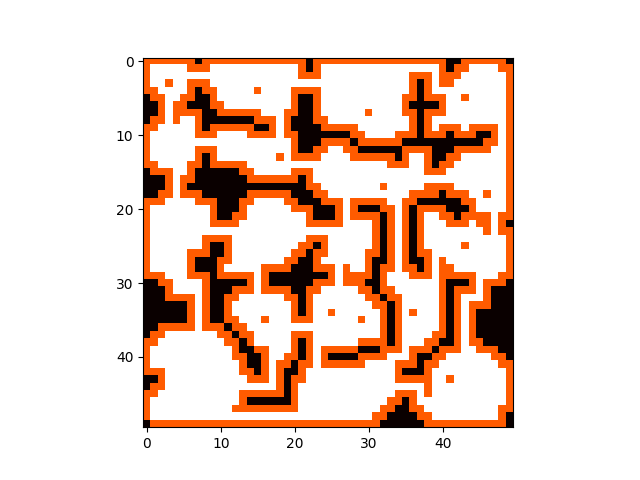
\includegraphics[scale=0.8]{images/map.png}
	\caption{Map}
	\label{fig:map}
\end{figure}

\begin{figure}[!ht]
	\centering
	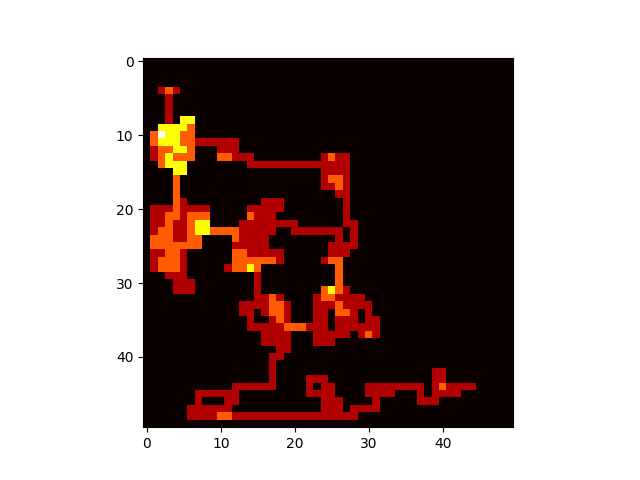
\includegraphics[scale=0.70]{images/test1_agent1.png}
	\caption{Agent 1}
	\label{fig:test1Agent1}
\end{figure}

\begin{figure}[!ht]
	\centering
	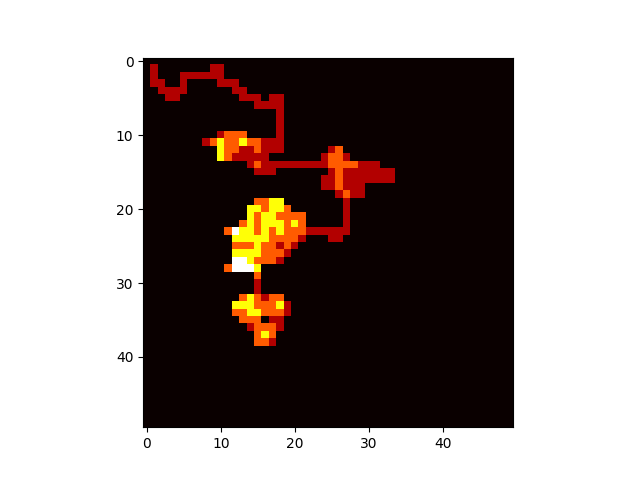
\includegraphics[scale=0.70]{images/test1_agent2.png}
	\caption{Agent 2}
	\label{fig:test1Agent2}
\end{figure}

\begin{figure}[!ht]
	\centering
	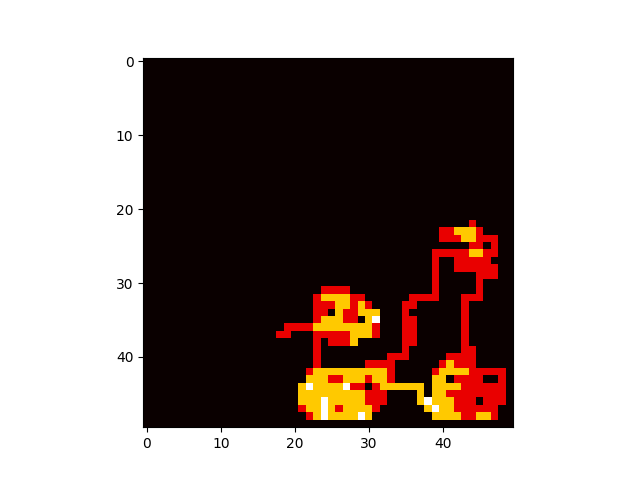
\includegraphics[scale=0.70]{images/test1_agent3.png}
	\caption{Agent 3}
	\label{fig:test1Agent3}
\end{figure}

\begin{figure}[!ht]
	\centering
	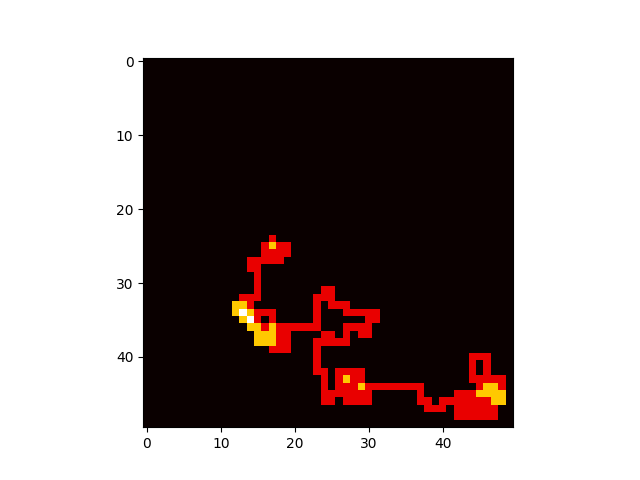
\includegraphics[scale=0.70]{images/test1_agent4.png}
	\caption{Agent 4}
	\label{fig:test1Agent4}
\end{figure}

\begin{figure}[!ht]
	\centering
	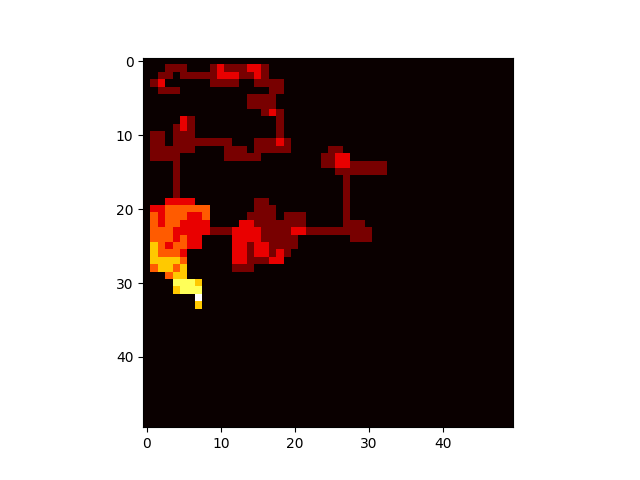
\includegraphics[scale=0.70]{images/test2_agent1.png}
	\caption{Agent 1}
	\label{fig:test2Agent1}
\end{figure}

\begin{figure}[!ht]
	\centering
	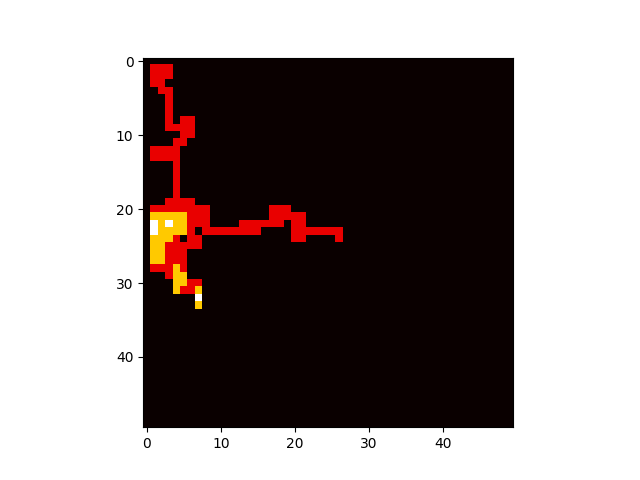
\includegraphics[scale=0.70]{images/test2_agent2.png}
	\caption{Agent 2}
	\label{fig:test2Agent2}
\end{figure}

\begin{figure}[!ht]
	\centering
	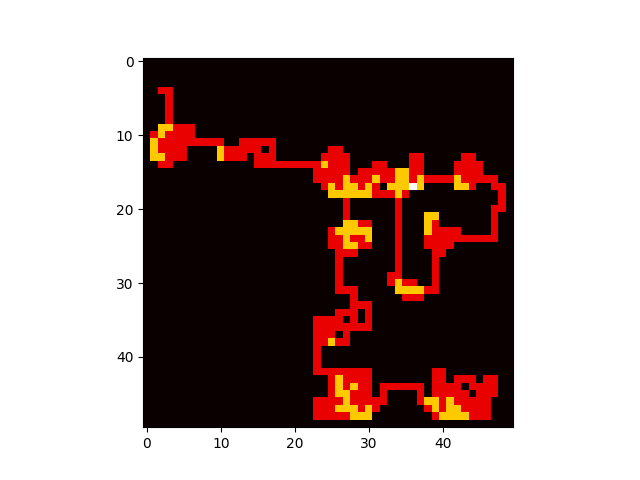
\includegraphics[scale=0.70]{images/test2_agent3.png}
	\caption{Agent 3}
	\label{fig:test2Agent3}
\end{figure}

\begin{figure}[!ht]
	\centering
	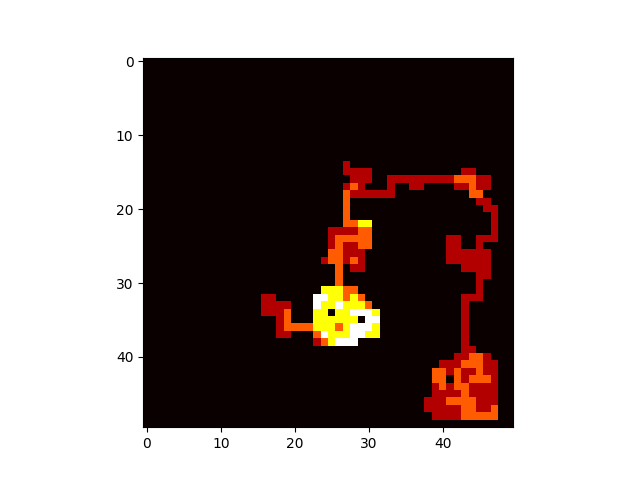
\includegraphics[scale=0.70]{images/test2_agent4.png}
	\caption{Agent 4}
	\label{fig:test2Agent4}
\end{figure}